\section{Problem Setting}


\begin{frame}
\frametitle{Numerical Methods for PDEs}
    Consider 2D problem:

    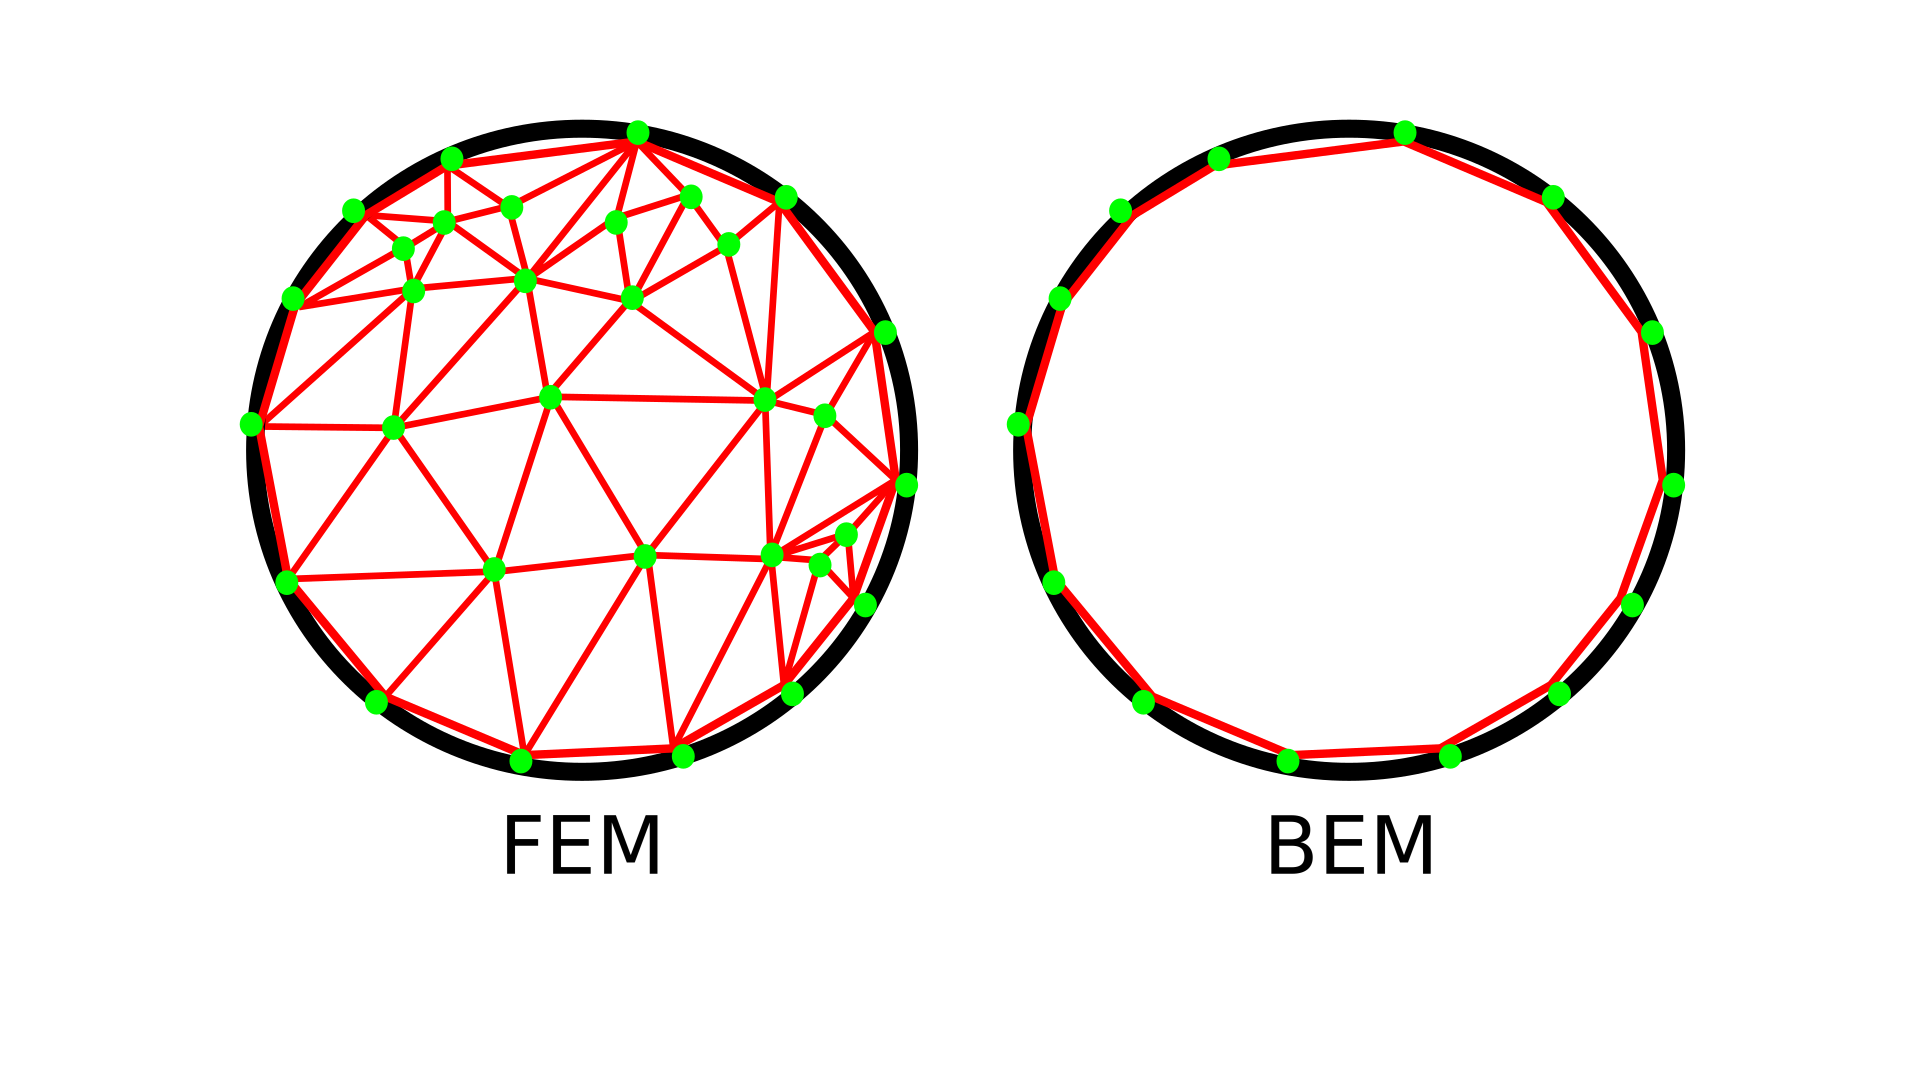
\includegraphics[width=\linewidth]{assets/fem_bem.pdf}
\end{frame}

\begin{frame}
    \frametitle{Laplace Interior Boundary Value Problem I}
    \begin{columns}
        \begin{column}{0.5\textwidth}

            Want to solve

            \begin{equation}
                \Delta u(x) = 0
            \end{equation}

            For $x \in \Omega$, with boundary $\partial \Omega$.


            \hspace*{5pt}

            Form an \textit{integral equation} using representation formula + boundary data.


        \end{column}

        \begin{column}{0.5\textwidth}

        \includegraphics[width=\linewidth]{assets/laplace.pdf}
        \end{column}
    \end{columns}
\end{frame}

\begin{frame}

    We seek $u \in C^2(\Omega) \cap C^2(\bar{\Omega})$ which satisfies $u=f$ on $\partial \Omega$.

    Let's write down a solution using a `double layer potential',

    $$u(x) = K \phi = \int_{\partial \Omega} \phi(y) \frac{\partial \Phi(x, y)}{\partial n (y)} ds(y), \> \> x \in \Omega$$

    $\phi(y)$ unknown surface density, $\Phi(x, y)$ fundamental solution. End up with \textit{boundary} integral equation,

    $$  \phi(x)  - 2 \int_\Gamma \phi(y) \frac{\partial \Phi(x, y)}{\partial n(y)} ds(y) = -2 f(x), \> \> x \in \Gamma $$

    $$ -\frac{1}{2} \phi + K \phi = f $$

    of the form

    $$ A\phi = f $$

    with $A = K - \frac{1}{2} I$


\end{frame}

\begin{frame}
    \textbf{Problem}: $A$ is \textit{dense}. Slow $O(N^2)$ application cost, $O(N^3)$ inversion cost. CPUs of the 1980s can't handle this.

    ...    But get to automatically incorporate boundary data \textit{and} get a reduction in problem dimension.

\end{frame}

\begin{frame}
    \textbf{Solution}: Hierarchical Solvers (Fast Multipole Method). Can apply in $O(N)$ (sometimes), and invert using Krylov methods.

    Workaround for slow computers!
\end{frame}


\begin{frame}
    \frametitle{Fast Multipole Methods I }
    \includegraphics[width=\linewidth]{assets/algorithm.pdf}

    Consider $N$ source and target particles,

    \begin{list}{-}{ }
        \item $O(N)$ boxes, so at least $O(N \log N)$ complexity.
    \end{list}

    FMM for Laplace is just $O(N)$, as number of boxes in interaction lists limited to constant number.

\end{frame}

\begin{frame}
    \frametitle{Fast Multipole Methods II }
    \includegraphics[width=\linewidth]{assets/three_step.png}
\end{frame}

% \begin{frame}
%     \frametitle{Fast Direct Solvers}
%     \includegraphics[width=\linewidth]{assets/ifmm.png}
%     \captionof*{figure}{ \scriptsize Ambisekaran, S \& Darve, E. \textit{The Inverse Fast Multipole Method}, arXiv:1407.1572v1 (2014)}

% \end{frame}

% \begin{frame}
%     \frametitle{Rusty Fast Solvers Project I}
%     \includegraphics[width=0.95\linewidth]{assets/rfs.png}
%     \captionof*{figure}{ \large https://github.com/rusty-fast-solvers}
% \end{frame}

% \begin{frame}
%     \frametitle{Rusty Fast Solvers Project II}

%     Checklist:

%     \begin{enumerate}
%         \item \color{green} Rusty Green Kernel  \color{black} - Optimized math kernel operations.
%         \item \color{green} Rusty Tree \color{black} - Distributed Octrees.
%         \item \color{green} Hyksort  \color{black} - Sorting algorithm for distributed arrays.
%         \item \color{orange} Rusty Compression \color{black} - Randomized compression library.
%         \item \color{orange} Rusty Field \color{black} - Field representations.
%         \item \color{red} Rusty FMM \color{black} - Fast Multipole Method.
%         \item \color{red} Rusty Inverse \color{black} - Fast Direct Solvers.
%     \end{enumerate}

% \end{frame}

% \begin{frame}
%     \frametitle{Rusty Fast Solvers Project III}

%     Rusty Tree is the most complete work item, with full Python bindings.

%     \hspace*{5pt}

%     It's a distributed octree implementation, parallelized with MPI.

%     \hspace*{5pt}

%     https://github.com/rusty-fast-solvers/rusty-tree

% \end{frame}